\section{Correcting the effect of photo-z quality cuts on galaxy clustering}
\label{sec:correction}

In the previous section we have seen that the photo-z quality cuts introduce extra clustering in the angular galaxy correlations, since they remove galaxies non-homogeneously from the sky. In this section, we want to find a way to correct for it.

We will use the framework presented in~\citet{Ho2012} and~\citet{Ross2011}, which the authors use for the treatment of systematic effects that influence the SDSS-III galaxy clustering, such as the stellar contamination, the sky brightness or the image quality of the instrument. 
Following~\citet{Ho2012} and~\citet{Ross2011}, the density fluctuation $\delta_i$ of the systematic effect $i$ modifies the true galaxy density fluctuation $\delta^t_g$ through a linear contribution modulated by $\epsilon_i$, so that the observed galaxy density fluctuation becomes:
\begin{equation}
\delta_g = \delta^t_g+\sum_{i}\epsilon_i \delta_i \label{delta_g_obs} \, ,
\end{equation}
where the contribution of the systematic effect must be small compared with $\delta^t_g$.

Therefore, assuming that there is no intrinsic cross-correlation between the true galaxy fluctuations and the systematic effect, $\langle \delta^t_g \delta_i \rangle = 0$, the cross-correlation between the observed galaxy density fluctuation and the systematic effect is:
\begin{equation}
\langle \delta_g \delta_i \rangle = \langle (\delta^t_g+\sum_{j}\epsilon_j \delta_j) \delta_i \rangle = \epsilon_i \langle \delta_i \delta_i \rangle + \sum_{j\neq i}\epsilon_j\langle \delta_j \delta_i \rangle \label{omega_god} \, .
\end{equation}
If we consider that the only systematic effect acting is the \textit{odds} distribution, the previous equations reduce to:
\begin{eqnarray}
\delta_g = \delta^t_g+\epsilon_{od} \delta_{od} \label{delta_g} \\
\langle \delta^t_g \delta_{od} \rangle = 0 \label{god_zero_2} \\
\langle \delta_g \delta_{od} \rangle = \epsilon_{od}\langle \delta_{od} \delta_{od} \rangle \label{omega_god_2} \, .
\end{eqnarray}
Then, the angular galaxy cross-correlation between two different galaxy maps, 1 and 2, at, for instance, different redshifts, is:
\begin{align}
\langle \delta_{g1} \delta_{g2} \rangle &= \langle (\delta^t_{g1}+\epsilon_{od1} \delta_{od1}) (\delta^t_{g2}+\epsilon_{od2} \delta_{od2}) \rangle \nonumber \\
&= \langle \delta^t_{g1} \delta^t_{g2} \rangle + \epsilon_{od1} \epsilon_{od2} \langle \delta_{od1} \delta_{od2} \rangle \nonumber \\ 
&= \langle \delta^t_{g1} \delta^t_{g2} \rangle + {\langle \delta_{g1} \delta_{od1} \rangle \over \langle \delta_{od1} \delta_{od1} \rangle }{ \langle \delta_{g2} \delta_{od2} \rangle \over \langle \delta_{od2} \delta_{od2} \rangle} \langle \delta_{od1} \delta_{od2} \rangle \, ,
\end{align}
where in the first equality we have used~(\ref{delta_g}), in the second~(\ref{god_zero_2}) and in the third~(\ref{omega_god_2}). What we measure is the left-hand side of the equation, and, therefore, we need to subtract the second term on the right-hand side to obtain the true values of the correlations. 

Therefore, the \textit{odds} correction for the angular cross-correlations of two different galaxy maps is:
\begin{equation}
\omega^t_{g1,g2}(\theta) = \omega_{g1,g2}(\theta) - {\omega_{g1,od1}(\theta) \over \omega_{od1,od1}(\theta)}{\omega_{g2,od2}(\theta)\over\omega_{od2,od2}(\theta)}\omega_{od1,od2}(\theta) \, ,
\label{12od_correction}
\end{equation}
where $\omega^t_{g1,g2}(\theta)\equiv \langle \delta^t_{g1} \delta^t_{g2} \rangle_\theta$ is the true galaxy cross-correlation, $\omega_{g1,g2}(\theta) \equiv \langle \delta_{g1} \delta_{g2} \rangle_\theta$ is the observed one, $\omega_{g1,od1}(\theta) \equiv \langle \delta_{g1} \delta_{od1} \rangle_\theta$ is the cross-correlation of the galaxies with the \textit{odds} in map 1 (the same for map 2), $\omega_{od1,od1}(\theta) \equiv \langle \delta_{od1} \delta_{od1} \rangle_\theta$ is the auto-correlation of the \textit{odds} in  map 1 (the same for map 2), and $\omega_{od1,od2}(\theta) \equiv \langle \delta_{od1} \delta_{od2} \rangle_\theta$ is the cross-correlation between the \textit{odds} maps 1 and 2.

If we were only interested in this correction for auto-correlations,
Eq.~(\ref{12od_correction}) would reduce to:
\begin{equation}
\omega^t_{g,g}(\theta) = \omega_{g,g}(\theta) - {\omega_{g,od}^2(\theta)\over\omega_{od,od}(\theta)} \, ,
\label{od_correction}
\end{equation}
where $\omega^t_{g,g}(\theta) \equiv \langle \delta^t_{g} \delta^t_{g} \rangle_\theta$ is the true galaxy auto-correlation, $\omega_{g,g}(\theta) \equiv \langle \delta_g \delta_g \rangle_\theta$ is the observed one, $\omega_{g,od}(\theta) \equiv \langle \delta_g \delta_{od} \rangle_\theta$ is the galaxy-\textit{odds} cross-correlation, and $\omega_{od,od}(\theta) \equiv \langle \delta_{od} \delta_{od} \rangle_\theta$ is the \textit{odds} auto-correlation.

The structure of Eqs.~(\ref{12od_correction}) and (\ref{od_correction}) is quite intuitive: we have the
correlations of the galaxies, shown on the top row of Figs.~\ref{auto_odcorr} and~\ref{cross_odcorr}, minus the cross-correlations of them with the photo-z quality, shown on the bottom row of~Fig.~\ref{gal_map}, properly normalized by the auto-correlations of the \textit{odds}.
Both $\omega_{g,g}(\theta)$ and $\omega_{g,od}(\theta)$ grow when the quality cuts are applied. Therefore, the increase in the auto-correlation will be compensated by the increase in the cross-correlation.

The origin of the galaxy-\textit{odds} cross-correlation is probably manifold. On the one hand,  
the \textit{odds} map can be seen as a proxy for other systematic effects, such as sky brightness, seeing, airmass, etc, and correcting for it, even without any photo-z quality cut, could therefore partially correct for these other systematic effects.
For this reason, we will also apply these corrections when no cut is applied.
On the other hand, in a galaxy catalog containing both early- and late-type galaxies (unlike Mega-Z, which contains almost exclusively early-type galaxies), the \textit{odds} corrections could also reflect the fact that early-type galaxies cluster more than late-type galaxies, and, at the same time, their photo-z quality tends to be better, thereby creating a cross-correlation between galaxy clustering and \textit{odds}. 

In~Eq.~(\ref{12od_correction}) the cross-correlations between different \textit{odds} maps, $\langle \delta_{od1} \delta_{od2} \rangle$, are needed. In our case, those are the maps on the top row of Fig.~{\ref{od_map}}. We compute all the cross-scorrelations and display them on Fig.~\ref{cross_od}. We see that all the \textit{odds} maps are cross-correlated with each other, at least up to angles $<10^\circ$. However, the higher the $z$, the lower the correlation. For example, the bins 1-2 are the most cross-correlated, while the bins 3-4 are the least. All the other combinations have similar values.  
\begin{figure}
\centering
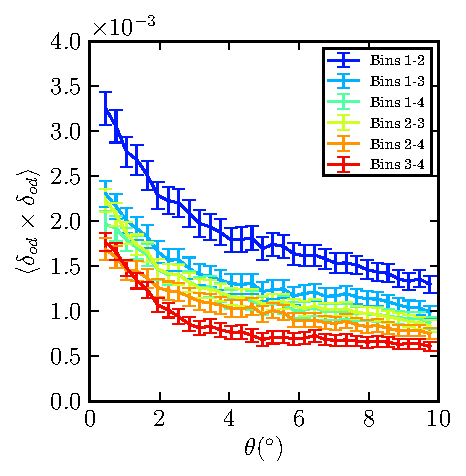
\includegraphics[width=80mm]{./plots/cross_od_plot.pdf}
\caption{All the possible combinations of the angular \textit{odds} cross-correlations between the different maps on the  top row of Fig~\ref{od_map}. They are needed for the \textit{odds} correction in~(\ref{12od_correction}). We see that all \textit{odds} maps are cross-correlated with each other, at least up to angles $<10^\circ$. However, the higher the $z$, the smaller the correlation.}
\label{cross_od}
\end{figure}

Finally, we apply the corrections to the measured angular galaxy clustering, before and after applying the photo-z quality cuts. 
The covariance $\text{Cov}_\omega(\theta_n , \theta_m )$ of the correlation functions after applying the \textit{odds} correction is obtained using Eq.~(\ref{covariance}) after applying the correction to each one of the jackknife correlation function $\omega_k(\theta_n)$.
The results are shown on the bottom rows of Fig.~\ref{auto_odcorr} for auto-correlations and Fig.~\ref{cross_odcorr} for cross-correlations. 
First, we see that the corrections work very well. After applying them, all measurements agree, regardless of the photo-z quality cut used in the analysis. 
Second, we see that the corrections not only work to remove the extra clustering introduced by the quality cuts, they also correct for any intrinsic extra clustering that might be present before any cut. For example, on the left-most plot of Fig.~\ref{auto_odcorr}, the auto-correlations were 1 or 2$\sigma$ above the prediction before any cut (blue). 
After applying the correction, most of the data points agree with their corresponding prediction.

The predictions in Fig.~\ref{auto_odcorr}, and most of those in Fig.~\ref{cross_odcorr} do not change much after the quality cuts, since they depend through (\ref{corr_prediction}) on the $N_i(z)$ functions in Fig.~\ref{Nz_bins},
which themselves change very little. In fact, the size of the measured error bars are not small enough to distinguish between different predictions. So much so that, although we have been able to correct for the extra clustering introduced by the quality cuts, the cuts themselves do not help in any relevant way in the clustering analysis, and, therefore, in this case there may be no obvious advantage in applying them. 
Furthermore, the relative errors in the corrected correlation functions can be substantially larger than those in the uncorrected ones: 
from a few percent larger to almost twice as large, depending on the angular scale, the photo-z bin and the value of the {\em odds} cut.

Things are different for cross-correlations. The strength of the signal of the cross-correlation between two different photo-z bins is mainly given by the amount of overlap in their $N_i(z)$, or, in other words, the fraction of galaxies that are at very similar true redshifts but, due to their photo-z uncertainty, end up in separate photo-z bins. In Fig.~\ref{Nz_bins}, we saw that the low tail of bin $0.6<z<0.65$, reduces considerably when the photo-z quality cuts are applied. Consequently, the overlap between this bin and the rest will also reduce, particularly the overlap with the farthest bin, $0.45<z<0.5$. This should result in differences in the predicted cross-correlations large enough to be distinguished by our measurements. If we look at the cross-correlation of the bins 1-4 on the top-right plot of Fig.~\ref{cross_odcorr}, we see that, at angles $<3^\circ$ where cross-correlations are not zero, the predicted curves differ more than the size of the error bars in the measurements. Even then, the corrections again put the measurements on top of their corresponding predicted curves. Note that, as for the auto-correlations, this is also true even when no {\em odds} cut is applied. This may have consequences for methods of photo-z calibration based on the study of the cross-correlations between photometric galaxy samples~\citep{Benjamin2010}.
